%-------------------------------------------------------------------------------
% 请勿删除本注释
% Free Response Question 2
%
% 指引:
% 如在小问之前有通用问题描述,请放置于此
%-------------------------------------------------------------------------------
\begin{figure}[H]
\centering
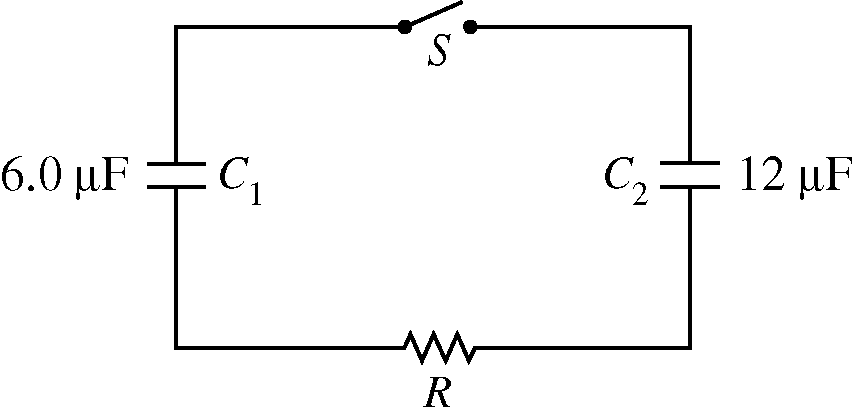
\includegraphics[scale=0.3]{images/img-018-044.png}
\end{figure}


\question
A $6.0 \mu \mathrm{F}$ capacitor, $C_{1}$, is initially charged using a $30 \mathrm{~V}$ battery. $C_{1}$ is then inserted in the circuit represented above with a resistor of resistance $R$ and the $12 \mu \mathrm{F}$ capacitor $C_{2}$, which is initially uncharged. The switch $S$ in the circuit is initially open. % 请删除并替换本行,与上一行 \question 之间不要留空行

\begin{parts}

%-------------------------------------------------------------------------------
% 请勿删除本注释
% Part (a)
%
% 指引:
% 如在小问之前有通用问题描述,请放置于此
%-------------------------------------------------------------------------------

\part
Calculate the charge $Q$ on $C_{1}$ before the switch is closed. % 请删除并替换本行,与上一行 \part 之间不要留空行

%-------------------------------------------------------------------------------
% 请勿删除本注释
% Part (b)
%
% 指引:
% 如在小问之前有通用问题描述,请放置于此
%-------------------------------------------------------------------------------

The switch is now closed.

\part
Let $q_{2}$ be the charge on capacitor $C_{2}$ at any time $t$ after the switch is closed. Write, but do NOT solve, a differential equation for the charge $q_{2}$ as a function of the time $t$. Write your equation in terms of the charge $Q$ from part (a), $C_{1}, C_{2}, R$, and fundamental constants, as appropriate. % 请删除并替换本行,与上一行 \part 之间不要留空行

%-------------------------------------------------------------------------------
% 请勿删除本注释
% Part (c)
%
% 指引:
% 如在小问之前有通用问题描述,请放置于此
%-------------------------------------------------------------------------------

\part
Calculate the final charges $Q_{1}$ and $Q_{2}$ on the two capacitors after equilibrium is reached. % 请删除并替换本行,与上一行 \part 之间不要留空行

%-------------------------------------------------------------------------------
% 请勿删除本注释
% Part (d)
%
% 指引:
% 如在小问之前有通用问题描述,请放置于此
%-------------------------------------------------------------------------------

\part
Calculate the energy dissipated in the circuit as the charge is redistributed. % 请删除并替换本行,与上一行 \part 之间不要留空行

%-------------------------------------------------------------------------------
% 请勿删除本注释
% Part (e)
%
% 指引:
% 如在小问之前有通用问题描述,请放置于此
%-------------------------------------------------------------------------------

\part
Suppose the resistor was replaced with one of larger resistance and the process was repeated. Would the time it takes capacitor $C_{2}$ to reach half its final charge now be longer, the same, or shorter than for the original circuit? % 请删除并替换本行,与上一行 \part 之间不要留空行

\underline{\qquad} Longer \qquad \underline{\qquad} The same \qquad  \underline{\qquad} Shorter

Justify your answer.

\end{parts}
